
\subsection{Web Business Skills}

To have a successful web business you need to know how to build a web application.  A web application typically has some interactive functionality that lets you order products.  The typical structure for this is an architecture like the following image:

\begin{comment}

for some reason the following section is killing the document

\begin{figure}[h!]
  \centering
  \fbox{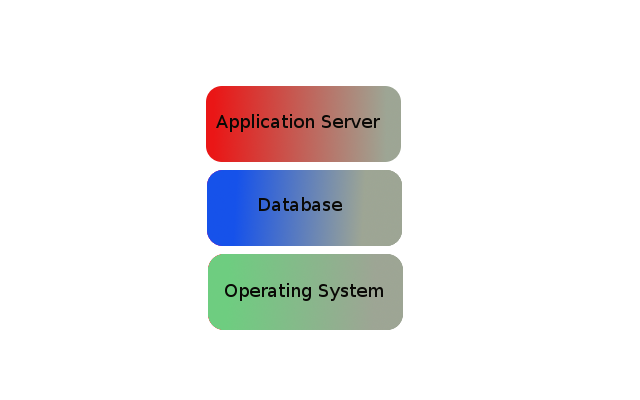
\includegraphics[width=130mm]{images/WebAppBasicArchitecture}}
  \caption{Basic Architecture}
\end{figure}

\end{comment}


\subsection{Application Server}

The application server is where all the code for your website lives.  This is where 90\% of your development effort will be spent.  You will write your web application in some \emph{Language} such as Java, PHP or Ruby, to name a few.  This application will store data, such as new orders, product catalog, etc..., in the Database.



You will want to learn the language you will use for your website.  You will also need to learn/understand web technologies such as: Cascading Style Sheets (CSS), Javascript, and HTML.

You will also need to learn to use the tools to write, manage and test your code.  These tools are an Integrated Development Environment (IDE), Version Control System (VCS) and bug tracker.

\subsection{Database}

The database contains your data.  Typically, we'll use either an Oracle database or MySQL.  The skills required for this are learning some basic SQL commands.





%%% Local Variables: 
%%% mode: latex
%%% TeX-master: "OnlineTailorStrategyBook"
%%% End: 
